\PassOptionsToPackage{unicode=true}{hyperref} % options for packages loaded elsewhere
\PassOptionsToPackage{hyphens}{url}
%
\documentclass[ignorenonframetext,]{beamer}
\usepackage{pgfpages}
\setbeamertemplate{caption}[numbered]
\setbeamertemplate{caption label separator}{: }
\setbeamercolor{caption name}{fg=normal text.fg}
\beamertemplatenavigationsymbolsempty
% Prevent slide breaks in the middle of a paragraph:
\widowpenalties 1 10000
\raggedbottom
\setbeamertemplate{part page}{
\centering
\begin{beamercolorbox}[sep=16pt,center]{part title}
  \usebeamerfont{part title}\insertpart\par
\end{beamercolorbox}
}
\setbeamertemplate{section page}{
\centering
\begin{beamercolorbox}[sep=12pt,center]{part title}
  \usebeamerfont{section title}\insertsection\par
\end{beamercolorbox}
}
\setbeamertemplate{subsection page}{
\centering
\begin{beamercolorbox}[sep=8pt,center]{part title}
  \usebeamerfont{subsection title}\insertsubsection\par
\end{beamercolorbox}
}
\AtBeginPart{
  \frame{\partpage}
}
\AtBeginSection{
  \ifbibliography
  \else
    \frame{\sectionpage}
  \fi
}
\AtBeginSubsection{
  \frame{\subsectionpage}
}
\usepackage{lmodern}
\usepackage{amssymb,amsmath}
\usepackage{ifxetex,ifluatex}
\usepackage{fixltx2e} % provides \textsubscript
\ifnum 0\ifxetex 1\fi\ifluatex 1\fi=0 % if pdftex
  \usepackage[T1]{fontenc}
  \usepackage[utf8]{inputenc}
  \usepackage{textcomp} % provides euro and other symbols
\else % if luatex or xelatex
  \usepackage{unicode-math}
  \defaultfontfeatures{Ligatures=TeX,Scale=MatchLowercase}
\fi
% use upquote if available, for straight quotes in verbatim environments
\IfFileExists{upquote.sty}{\usepackage{upquote}}{}
% use microtype if available
\IfFileExists{microtype.sty}{%
\usepackage[]{microtype}
\UseMicrotypeSet[protrusion]{basicmath} % disable protrusion for tt fonts
}{}
\IfFileExists{parskip.sty}{%
\usepackage{parskip}
}{% else
\setlength{\parindent}{0pt}
\setlength{\parskip}{6pt plus 2pt minus 1pt}
}
\usepackage{hyperref}
\hypersetup{
            pdftitle={Principe des méthodes de Monte Carlo},
            pdfauthor={Pierre Gloaguen},
            pdfborder={0 0 0},
            breaklinks=true}
\urlstyle{same}  % don't use monospace font for urls
\newif\ifbibliography
\usepackage{graphicx,grffile}
\makeatletter
\def\maxwidth{\ifdim\Gin@nat@width>\linewidth\linewidth\else\Gin@nat@width\fi}
\def\maxheight{\ifdim\Gin@nat@height>\textheight\textheight\else\Gin@nat@height\fi}
\makeatother
% Scale images if necessary, so that they will not overflow the page
% margins by default, and it is still possible to overwrite the defaults
% using explicit options in \includegraphics[width, height, ...]{}
\setkeys{Gin}{width=\maxwidth,height=\maxheight,keepaspectratio}
\setlength{\emergencystretch}{3em}  % prevent overfull lines
\providecommand{\tightlist}{%
  \setlength{\itemsep}{0pt}\setlength{\parskip}{0pt}}
\setcounter{secnumdepth}{0}

% set default figure placement to htbp
\makeatletter
\def\fps@figure{htbp}
\makeatother

\newcommand{\rmd}{\text{d}}
\newcommand{\R}{\mathbb{R}}
\newcommand{\E}{\mathbb{E}}
\newcommand{\Unif}{\mathcal{U}}

\title{Principe des méthodes de Monte Carlo}
\author{Pierre Gloaguen}
\date{22/03/2020}

\begin{document}
\frame{\titlepage}

\begin{frame}{Exemple introductif (1)}
\protect\hypertarget{exemple-introductif-1}{}

Soit \(g\) une fonction sur \(\mathbb{R}\) et \(a < b\) deux réels.

Supposons que l'on souhaite calculer une intégrale (finie) du type
\[I = \int_a^b g(x) \text{d}x\]

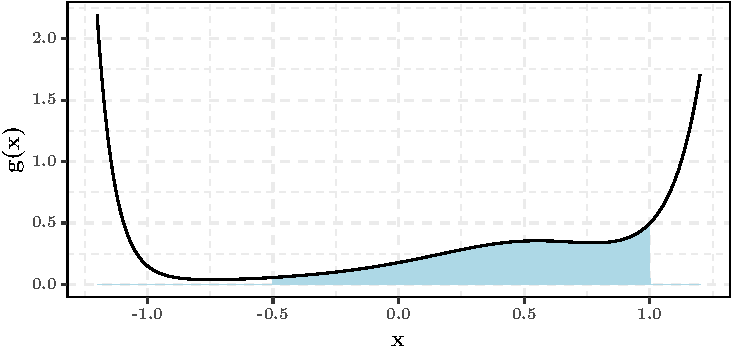
\includegraphics{diapos_monte_carlo_files/figure-beamer/plot_phi-1.pdf}

\end{frame}

\begin{frame}{Exemple introductif (2)}
\protect\hypertarget{exemple-introductif-2}{}

\[\begin{array}{rl}
  I &= \int_a^b g(x) \text{d}x\\
  \pause
  &=  \int_{\mathbb{R}} \overbrace{(b - a) g(x)}^{:= \varphi(x)} \frac{\mathbf{1}_{a\leq x\leq b}}{b - a}\text{d}x\\
  \pause
  &= \mathbb{E}[\varphi(X)], \text{ où } X\sim\mathcal{U}[a,b].
  \end{array}\] \pause

\textbf{Estimateur de Monte Carlo}

On fixe un entier \(M > 0\). On simule un échantillon \(X_1,\dots, X_M\)
selon \(X\sim\mathcal{U}[a,b]\), on pose alors l'estimateur:
\[\hat{I}_M = \frac{1}{M}\sum_{k = 1}^M \varphi(X_k)\] \pause

\textbf{Remarques}

\begin{itemize}
\tightlist
\item
  \(M\) est appelé \textbf{effort de Monte Carlo};
\item
  On suppose pour le moment qu'on \textbf{sait simuler selon
  \(\mathcal{U}[a,b]\)};
\item
  L'estimateur de \(I\) est une \textbf{variable aléatoire}.
\end{itemize}

\end{frame}

\begin{frame}{Exemple introductif (3)}
\protect\hypertarget{exemple-introductif-3}{}

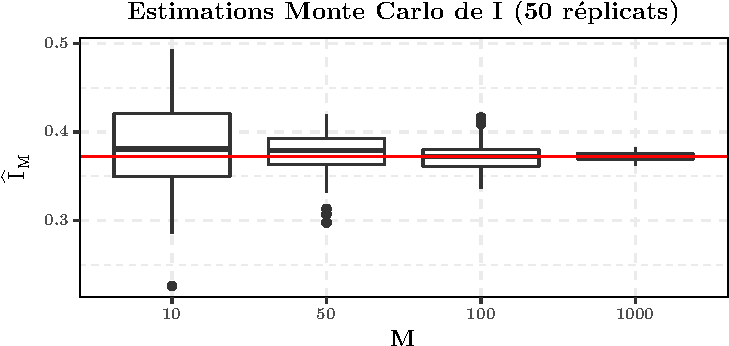
\includegraphics{diapos_monte_carlo_files/figure-beamer/monte_carlo_estimate_ex1-1.pdf}

\end{frame}

\begin{frame}{Cas générique}
\protect\hypertarget{cas-guxe9nuxe9rique}{}

On veut calculer une intégrale
\[I = \int_{\mathbb{R}^d} \varphi(x) f(x) \text{d}x\] où \(f\) est une
fonction positive, telle que \(\int_{\mathbb{R}^d} f(x)\text{d}x = 1\),
alors on se sert du fait que \[
I = \mathbb{E}[\varphi(X)]
\] où \(X\) est une variable aléatoire de densité \(f\).

\textbf{Estimateur de Monte Carlo}

On fixe un entier \(M > 0\). On simule un échantillon \(X_1,\dots, X_N\)
selon \(X\sim f(\cdot)\), on pose alors l'estimateur:
\[\hat{I}_N = \frac{1}{M}\sum_{k= 1}^M \varphi(X_k)\]

\end{frame}

\begin{frame}{Pourquoi?}
\protect\hypertarget{pourquoi}{}

Les \(\varphi(X_1),\dots,\varphi(X_N)\) sont des variables aléatoires
i.i.d. d'espérance \(\mathbb{E}[\varphi(X)]\) finie, avec
\(X\sim f(\cdot)\). \pause

Loi des grands nombres:
\[\frac{\varphi(X_1) + \dots + \varphi(X_N)}{M} \underset{M\rightarrow\infty}{\overset{\text{p.s.}}{\longrightarrow}} \mathbb{E}[\varphi(X)]\]

\end{frame}

\begin{frame}{Propriétés}
\protect\hypertarget{propriuxe9tuxe9s}{}

\textbf{Sans biais}
\[\mathbb{E}[\hat{I}_N] = \frac{1}{M}\sum_{k = 1}^M \mathbb{E}[\varphi(X_k)] \overset{\text{id. distrib}}{=} \mathbb{E}[\varphi(X)] = I\]
\pause \textbf{Variance} Si \(\mathbb{V}[\varphi(X)] < \infty\)
\[\mathbb{V}[\hat{I}_N] \overset{\text{ind.}}{=} \frac{1}{M^2}\sum_{k = 1}^M \mathbb{V}[\varphi(X_k)] \overset{\text{id. distrib}}{=} \frac{1}{M} \mathbb{V}[\varphi(X)]\]
\pause \textbf{Loi} La loi des grands nombres nous donne la loi
asymptotique
\[\sqrt{M}\left(\hat{I}_N - I \right) \underset{M\rightarrow\infty}{\overset{\text{Loi}}{\longrightarrow}} \mathcal{N}(0, \mathbb{V}[\varphi(X)])\]

\end{frame}

\begin{frame}{Loi de l'estimateur}
\protect\hypertarget{loi-de-lestimateur}{}

\begin{itemize}
\tightlist
\item
  100 réplicats d'échantillons Monte Carlo de taille \(M = 1000\).
\end{itemize}

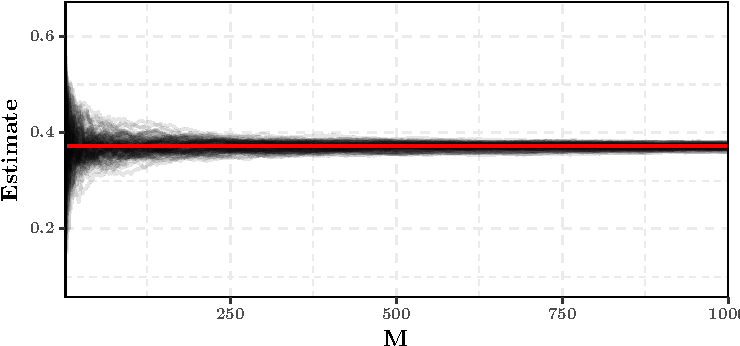
\includegraphics{diapos_monte_carlo_files/figure-beamer/plot_all_estimates-1.pdf}

\end{frame}

\begin{frame}{Intervalle de confiance}
\protect\hypertarget{intervalle-de-confiance}{}

On note \[\sigma^2 = \mathbb{V}[\varphi(X)].\]

Ainsi, en notant \(z_{\alpha}\) le quantile d'ordre \(\alpha \in]0, 1[\)
de la loi \(\mathcal{N} (0, 1)\), si on définit l'intervalle aléatoire
\[J_M = \left[\hat{I}_M - z_{1 - \alpha/2}\sqrt{\frac{\sigma^2}{M}}; \hat{I}_M + z_{1 - \alpha/2}\sqrt{\frac{\sigma^2}{M}}\right]\]
Alors,
\[\mathbb{P}(J_M \ni I) \underset{M\rightarrow \infty}{\longrightarrow} 1-\alpha\]

\(J_M\) est donc un intervalle de confiance asymptotique au niveau 1 -
\(\alpha\) pour la valeur de \(I\).

\end{frame}

\begin{frame}{Intervalle de confiance (2)}
\protect\hypertarget{intervalle-de-confiance-2}{}

En pratique cependant, cet intervalle n'est pas calculable car
\(\sigma^2\) est inconnu

On dispose cependant d'un estimateur consistant de \(\sigma^2\) donné
par
\[\hat{\sigma}^2_M = \frac{1}{M}\sum_{k = 1}^M \left(\varphi(X_k) - \hat{I}_M\right)^2\]

\begin{itemize}
\tightlist
\item
  Dans l'expression précédente, on remplace \(\sigma^2\) par son
  estimateur.
\item
  Le lemme de Slutski nous assure que les propriétés de \(J_M\) restent
  vraies.
\end{itemize}

\end{frame}

\begin{frame}{Intervalle de confiance (3)}
\protect\hypertarget{intervalle-de-confiance-3}{}

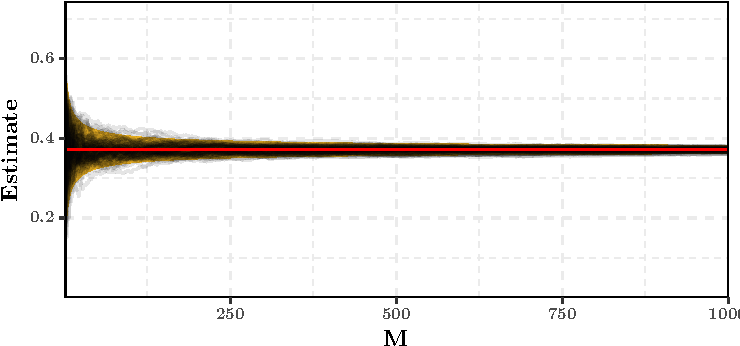
\includegraphics{diapos_monte_carlo_files/figure-beamer/plot_IC-1.pdf}

\end{frame}

\begin{frame}{Comparaison avec l'intégration numérique}
\protect\hypertarget{comparaison-avec-lintuxe9gration-numuxe9rique}{}

L'objectif présenté ici est de calculer, en dimension \(d\), une
intégrale: \[\int_{\mathbb{R}^d} g(x) \text{d}x\] - Calcul possible par
méthode numérique (méthode des cubes).\pause

\begin{itemize}
\tightlist
\item
  \textbf{Intégration numérique:} Pour une fonction \(g\) de classe
  \(C^s\), l'erreur est de l'ordre \(\frac{1}{M^{\frac{s}{d}}}\) (où
  \(M\) est le nombre d'évaluations de la fonction).

  \begin{itemize}
  \tightlist
  \item
    Il faut connaître la régularité de \(g\)!
  \item
    L'erreur augmente avec la dimension.\pause
  \end{itemize}
\item
  \textbf{Méthodes Monte Carlo:} Pour les méthodes de Monte Carlo,
  l'écart type de l'erreur est de l'ordre \(\frac{1}{M^{\frac{1}{2}}}\).

  \begin{itemize}
  \tightlist
  \item
    Indépendamment de la régularité de \(g\)!
  \item
    Indépendamment de la dimension!
  \end{itemize}
\end{itemize}

Ainsi, ces méthodes deviennent vite avantageuses quand \(d\) est grand.

\end{frame}

\end{document}
